% \documentclass[10pt]{beamer}
\documentclass[9pt, aspectratio=169]{beamer}
\usepackage[utf8]{inputenc}
\usepackage[T1]{fontenc}
%\usepackage{lmodern}
\usepackage{amsfonts,amssymb,amsmath}
\usepackage[english]{babel}
\usetheme{Frankfurt}

\usepackage{csquotes}
\usepackage{setspace}

\usepackage{colortbl}
\usepackage{tabularx}
\renewcommand\tabularxcolumn[1]{m{#1}}

\usepackage{booktabs}
\usepackage{amssymb}
\usepackage{pifont}
\usepackage[inkscapeformat=png]{svg}
\usepackage{graphicx}
\usepackage{times}
\setbeamertemplate{caption}[numbered]
% \setbeamertemplate{bibliography item}{[\theenumiv]}
\setbeamertemplate{bibliography item}[text]

\setbeamerfont{bibliography item}{size=\tiny}
\setbeamerfont{bibliography entry author}{size=\tiny}
\setbeamerfont{bibliography entry title}{size=\tiny}
\setbeamerfont{bibliography entry location}{size=\tiny}
\setbeamerfont{bibliography entry note}{size=\tiny}

% \setbeamerfont{frametitle}{size=\large}

\usepackage{ragged2e}
\setbeamercolor{section in foot}{fg=white,bg=darkorange}
\setbeamercolor{subsection in foot}{fg=white,bg=darkorange}
\setbeamercolor{frametitle}{fg=white, bg=darkorange}
\setbeamercolor{title}{fg=white, bg=darkorange}
\setbeamercolor{frame}{bg=darkorange}
\setbeamercolor{block title}{bg=darkorange,fg=white}

\setbeamercolor{item}{fg=darkorange}

% \definecolor{darkorange}{rgb}{0.81, 0.52, 0.05}
\definecolor{darkorange}{rgb}{1,0.5,0}
\definecolor{darkorange2}{rgb}{1, 0.64, 0.2}
\definecolor{honeydew}{rgb}{1, 0.85, 0.45}


\newenvironment{variableblock}[3]{%
  \setbeamercolor{block body}{#2}
  \setbeamercolor{block title}{#3}
  \begin{block}{#1}}{\end{block}}

\newenvironment{prosblock}[1]{%
  % \setbeamercolor{block body}{bg=blue,fg=white}
  \setbeamercolor{block title}{bg=blue,fg=white}
  \begin{block}{#1}}{\end{block}}

\newenvironment{consblock}[1]{%
  % \setbeamercolor{block body}{bg=red,fg=white}
  \setbeamercolor{block title}{bg=red,fg=white}
  \begin{block}{#1}}{\end{block}}

\newcommand{\cmark}{\ding{51}}%
\newcommand{\xmark}{\ding{55}}%

\renewcommand{\arraystretch}{1.5}

% ==========================

\begin{document}

\author{\textbf{Julien Soulé}, Jean-Paul Jamont, Michel Occello, Paul Théron, Louis-Marie Traonouez}

\title{\textbf{Towards a Multi-Agent Simulation of Cyber-attackers and Cyber-defenders Battles}}

\subtitle{SMC 2023 Presentation}

% \logo{
\includegraphics[scale=0.01]{figures/grenoble-inp_logo.png}}

\institute{\footnotesize \textit{University Grenoble Alpes, Grenoble
INP, LCIS, 26000, Valence, France \\
julien.soule@lcis.grenoble-inp.fr}}

\date{\textit{\footnotesize \today}}

%\subject{}
\setbeamercovered{transparent}
%\setbeamertemplate{navigation symbols}{}
\begin{frame}[plain]
	\maketitle\vspace{-0.8cm}
	\begin{figure}[ht!]
		\centering
            
\includegraphics[height=0.8cm]{figures/la-ruche_logo.png}
            \hspace{0.8cm}
            
\includegraphics[height=0.8cm]{figures/lcis_logo.png}
            \hspace{0.8cm}
		
\includegraphics[height=0.8cm]{figures/grenoble-inp_logo.png}
            \hspace{0.8cm}
            
\includegraphics[height=0.8cm]{figures/uga_logo.jpg}
	\end{figure}
\end{frame}

\begin{frame}{Content}
	\tableofcontents
\end{frame}

\AtBeginSection[]{
	\begin{frame}
		\frametitle{}
		\tableofcontents[currentsection]
	\end{frame}
}

%%%%%%%%%%%%%%%%%%%%%%%%%%%%%%%%%%%%

	\section{Introduction}
	\begin{frame}[allowframebreaks]{Introduction}

	   \begin{block}{AICA: Autonomous Intelligent Cyberdefense Agent \cite{theron_autonomous_2021}}

            An agent theorized by « IST-152 NATO » between 2016-2019 that is to be deployed on networked nodes to:
 
	       \begin{itemize}
                \item Detect, identify and characterize anomalies/attacks
                \item Plan and execute countermeasures
                \item Communicate with C2, operators\dots
                \item Being autonomous, stealthy, inter-operable, able to learn
		\end{itemize}

        \end{block}

        \begin{block}{MASCARA: Multi Agent System Centric AICA Reference Architecture \cite{theron_autonomous_2021}}
            \begin{itemize}
                \item A multi-agent vision of a decentralized and distributed AICA;
                \item A set of collaborative cyber-defenders fighting back against cyber-attacker(s) deployed over a networked system.
            \end{itemize}
        \end{block}

        \begin{alertblock}{Main concerns}
            No available consistent, clear and general framework to deal with cyber-defenders fighting against cyber-attackers in a networked system:
            \begin{itemize}
                \item Need to clarify how agents, environment and their interactions should be envisioned consistently;
                \item Need to assess collective cyber-defense experimentally through various criteria.
            \end{itemize}

        \end{alertblock}

        \begin{block}{Intended contributions}
            \begin{itemize}
                \item A formal model for cyber-defenders fighting against cyber-attackers in a networked system;
                \item A simulation tool to assess the efficiency of cyber-defenders / cyber-attackers collective actions for various attack scenarios.
            \end{itemize}
        \end{block}
 
	\end{frame}
% \AtBeginSection[]{
% 	\begin{frame}
% 		\frametitle{}
% 		\tableofcontents[currentsection]
% 	\end{frame}
% }

%%%%%%%%%%%%%%%%%%%%%%%%%%%%%%%%%%%%
 
 \section{Models for \textquote{cyber-attackers vs. cyber-defenders} and gaps}
 
	% \subsection{Related works}
 
	% \begin{frame}{Related works}
	% 	{Attack graphs}

 %            \begin{block}{Attack graphs~\cite{CPhilips1998}}
 %                Graphical representation of the system as a set of nodes and the possible attacks as edges between those nodes.
 %            \end{block}

 %            \begin{prosblock}{Main pros}
 %                \begin{itemize}
 %                    \item Formalization: vulnerabilities imply expressing concretely the consequences on the network.
 %                \end{itemize}
 %            \end{prosblock}

 %            \begin{consblock}{Main cons}
 %                \begin{itemize}
 %                    \item No defense: cyber-defense is not properly taken into account.
 %                \end{itemize}
 %            \end{consblock}
 
	% \end{frame}

	% \begin{frame}{Related works}
	% 	{Attack-Defense trees}

 %            \begin{block}{Attack-Defense trees~\cite{BKordy2010}}
 %                Graphical models representing the attacker's goals and the defender's countermeasures as a tree structure.
 %            \end{block}

 %            \begin{prosblock}{Main pros}
 %                \begin{itemize}
 %                    \item Attack and defense: cyber-attackers' actions can be decorated with defender's countermeasures;
 %                    \item High genericity: suited for various scenarios.
 %                \end{itemize}
 %            \end{prosblock}

 %            \begin{consblock}{Main cons}
 %                \begin{itemize}
 %                    \item Low detail level: too abstract for a comprehensive understanding of the impacts of action on the environment.
 %                \end{itemize}
 %            \end{consblock}

	% \end{frame}

	% \begin{frame}{Related works}
	% 	{Petri nets model}

 %            \begin{block}{Petri nets model}
 %                As Petri nets can be used to describe concurrent processes, it is possible to model attackers and defenders in a networked system such as in \textquote{Mirai vs white worm}~\cite{SYamaguchi2020}
 %            \end{block}

 %            \begin{prosblock}{Main pros}
 %                \begin{itemize}
 %                    \item High formalization: possible to simulate precisely a battle between cyber-defenders and cyber-attackers. 
 %                \end{itemize}
 %            \end{prosblock}

 %            \begin{consblock}{Main cons}
 %                \begin{itemize}
 %                    \item No ready to use framework: requires spending time on modeling for each context;
 %                    \item High complexity: difficult to get an overall picture for large systems.
 %                \end{itemize}
 %            \end{consblock}

	% \end{frame}

	% \begin{frame}{Related works}
	% 	{Game models}

 %            \begin{block}{Game models}
 %                Envisioned \textquote{Game theoretical} models include: \textquote{Partially Observable Stochastic Game} (POSG) and \textquote{Decentralized Partially Observable Markov Decision Process} (Dec-POMDP)~\cite{beynier2010}.

 %            \end{block}

 %            \begin{prosblock}{Main pros}
 %                \begin{itemize}
 %                    \item Formalization: both POSGs and Dec-POMDPs are mathematical modeling of decision-making problems;
 %                    \item Collaborative oriented: in a Dec-POMDP, agents receive a common reward to achieve a common goal~\cite{bernstein2013}.
 %                \end{itemize}
 %            \end{prosblock}

 %            \begin{consblock}{Main cons}
 %                \begin{itemize}
 %                    \item No ready to use framework: requires spending time on modeling for each context;
 %                    % \item Individual oriented: in a POSG, agents may have different goals as each agent has its own reward function~\cite{jk2020}.
 %                \end{itemize}
 %            \end{consblock}

	% \end{frame}

        % \subsection{Theoretical and technical gap}
        \begin{frame}{Models for \textquote{cyber-attackers vs. cyber-defenders} and gaps}
            {}

            \setstretch{0.1}

            \begin{table}
        
                \begin{tabularx}{\linewidth}{
                >{\centering\arraybackslash\hsize=0.7\hsize}X
                >{\centering\arraybackslash\hsize=0.5\hsize}X
                >{\centering\arraybackslash\hsize=0.5\hsize}X
                >{\centering\arraybackslash\hsize=0.5\hsize}X
                >{\centering\arraybackslash\hsize=0.5\hsize}X
                >{\centering\arraybackslash\hsize=0.5\hsize}X
                }
                \toprule
            
                { {\textbf{}}}
                & {\textbf{\scriptsize Attack \& Defense}}
                & {\textbf{\scriptsize Genericity}}
                & {\textbf{\scriptsize Formalization}}
                & {\textbf{\scriptsize Collaborative oriented}}
                & {\textbf{\scriptsize Practicality}}
    
                \\ \midrule
                
                {  \textbf{\scriptsize Attack graphs} }
                & { \scriptsize  only attack  }
                & { \scriptsize  medium }
                & { \scriptsize  medium }
                & { \scriptsize  no }
                & { \scriptsize  medium }
    
                \\
                \\
                \\

                {  \textbf{\scriptsize AD trees} }
                & { \scriptsize  both }
                & { \scriptsize  good }
                & { \scriptsize  medium }
                & { \scriptsize  possible }
                & { \scriptsize  good }
    
                \\
                \\
                \\

                {  \textbf{\scriptsize Petri nets} }
                & { \scriptsize  both possible }
                & { \scriptsize  good }
                & { \scriptsize  good }
                & { \scriptsize  possible }
                & { \scriptsize  low }
    
                \\
                \\
                \\

                {  \textbf{\scriptsize Game theory (Dec-POMDP)} }
                & { \scriptsize  both possible }
                & { \scriptsize  good }
                & { \scriptsize  good }
                & { \scriptsize  possible }
                & { \scriptsize  good }
    
                \\
                
                \bottomrule
                    
                \end{tabularx}
            
            \end{table}

            \setstretch{1}

            \begin{block}{Theoretical and technical gaps}
                \begin{itemize}
                    \item Taking into account both cyber-attackers and collaborative cyber-defenders;
                    \item Having a adaptative formalization allowing to implement it in highly evolving real context while keeping being practical.
                \end{itemize}
            \end{block}

            Yet Dec-POMDP is close and can be extended to meet our needs\dots
  
	\end{frame}
% \AtBeginSection[]{
% 	\begin{frame}
% 		\frametitle{}
% 		\tableofcontents[currentsection]
% 	\end{frame}
% }

%%%%%%%%%%%%%%%%%%%%%%%%%%%%%%%%%%%%
 
 \section{Formal model and simulation}

        \subsection{Formal model for \textquote{cyber-attackers vs. cyber-defenders}}
        
 	\begin{frame}{Formal model for \textquote{cyber-attackers vs. cyber-defenders}}
		{Decentralized Partially Observable Markov Decision Process}

            Receiving last observations and reward from previous iteration and choosing next action.

            \begin{figure}
                \centering
                \includesvg[width=1.05\textwidth]{figures/model_illustration_1.svg}
            \end{figure}
  
	\end{frame}

 	\begin{frame}{Formal model for \textquote{cyber-attackers vs. cyber-defenders}}
		{Decentralized Partially Observable Markov Decision Process}

            Applying chosen actions to change environment properties.

            \begin{figure}
                \centering
                \includesvg[width=1.05\textwidth]{figures/model_illustration_2.svg}
            \end{figure}
  
	\end{frame}

 	\begin{frame}{Formal model for \textquote{cyber-attackers vs. cyber-defenders}}
		{Decentralized Partially Observable Markov Decision Process}

            Next iteration: receiving new observations and choosing action\dots

            \begin{figure}
                \centering
                \includesvg[width=0.65\textwidth]{figures/model_illustration_3.svg}
            \end{figure}

            \vspace{-0.1cm}

            Ends when maximum iteration number or attack goal is reached.
  
	\end{frame}

        \subsection{Simulation implementation}
	% \begin{frame}{Simulation implementation}
 %            {Available simulation works}

 %            \begin{block}{Potential \textquote{ready to use} simulators}
 %                \begin{itemize}
 %                    \item \textit{NeSSi2}~\cite{DGrunewald2011}: an agent-based simulation platform aiming to model only packet-level description of a networked system and the effects of DDoS attacks;
 %                    \item Kotenko et al.~\cite{IKotenko2007} relies on \textit{OMNet++}~\cite{Varga2010} to model and simulate cooperative cyber-defense agents against network attacks.
 %                \end{itemize}
 %            \end{block}
            
 %            However, among these, none can fully meet both the consideration of a multi-agent cyber environment for a Dec-POMDP model.

 %            \begin{block}{Tools towards implementing}
 %                \begin{itemize}
 %                    \item Extending discrete-event simulators such as \textit{CYST}\cite{drasar_session-level_2020} or \textit{CyberBattleSim}~\cite{cyberbattlesim} for multi-agent context
 %                    \item Using \textit{PettingZoo}~\cite{jk2020} which is a platform designed to implement a Dec-POMDP model
 %                \end{itemize}
 %            \end{block}
      
	% \end{frame}


        \begin{frame}{Model implementation as a simulation}
            {}

            No available simulator fully meet both the consideration of a multi-agent cyber environment for a Dec-POMDP model but\dots

            \begin{itemize}
                \item Extending discrete-event simulators such as \textit{CYST}\cite{drasar_session-level_2020} or \textit{CyberBattleSim}~\cite{cyberbattlesim} for multi-agent context
                \item Using \textit{PettingZoo}~\cite{jk2020} which is a platform designed to implement a Dec-POMDP model
            \end{itemize}

            \

            \begin{block}{Multi Cyber Agent Simulator (MCAS)~\cite{MCASWebsite}}

                \begin{itemize}
                    \item Loading/saving a scenario file describing the nodes properties, actions of the environment and the defined agents with their behaviors;
                    \item Executing the agents of this environment in turn-by-turn mode via the API or graphical interface;
                    \item Viewing the environment and metrics.
                \end{itemize}

            \end{block}

        \end{frame}

        
        \begin{frame}{Model implementation as a simulation}
            {}

            \begin{figure}
                \centering
                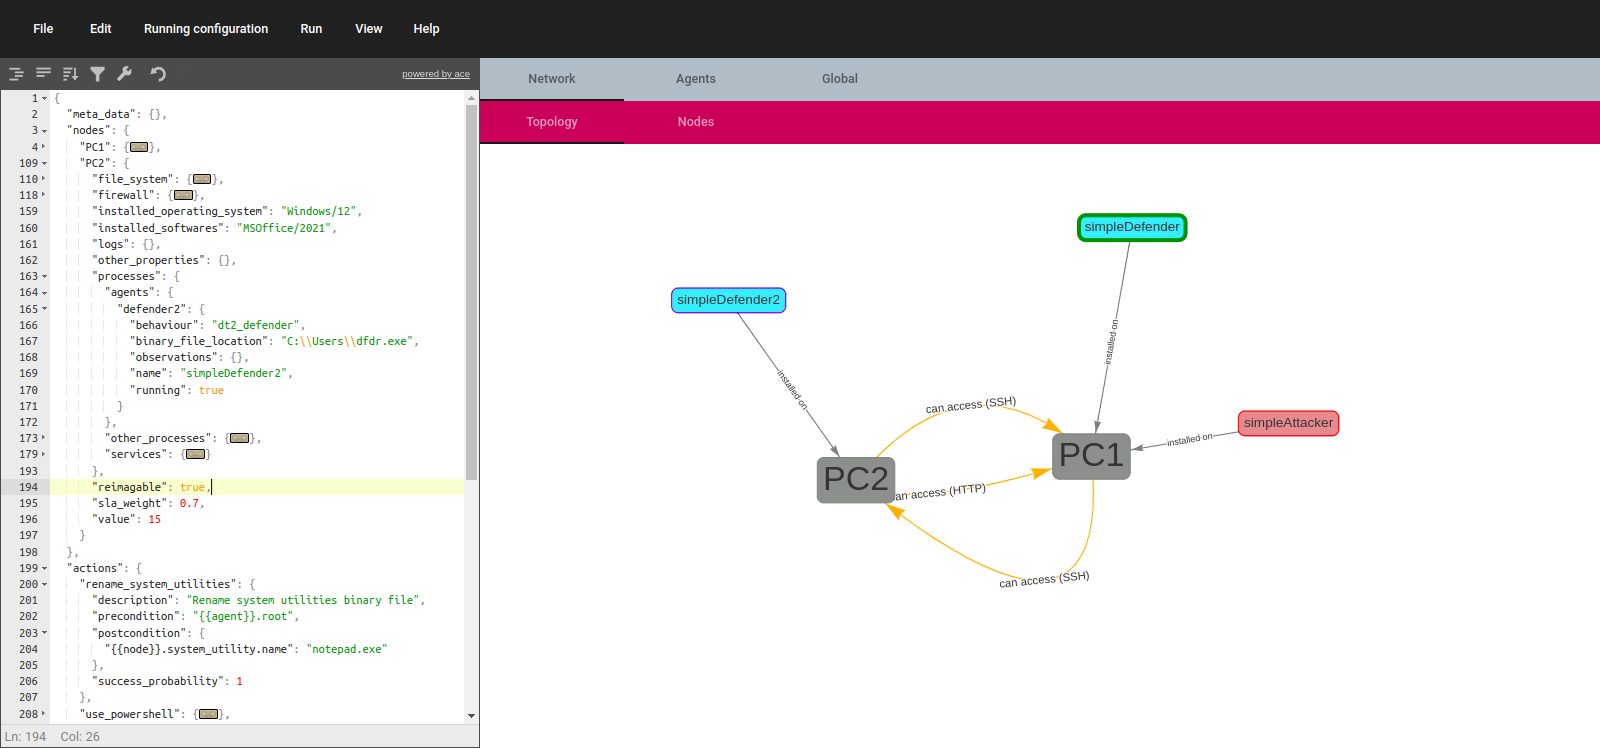
\includegraphics[width=0.95\textwidth]{figures/interface_MCAS.png}
                \caption{Overview of the MCAS interface}
                \label{fig:interface_simulateur}
            \end{figure}
        
        \end{frame}

        % \begin{frame}{Simulation implementation}
        %     {MCAS: Multi Cyber Agent Simulator}
        
        %     \begin{center}
        %             \embedvideo{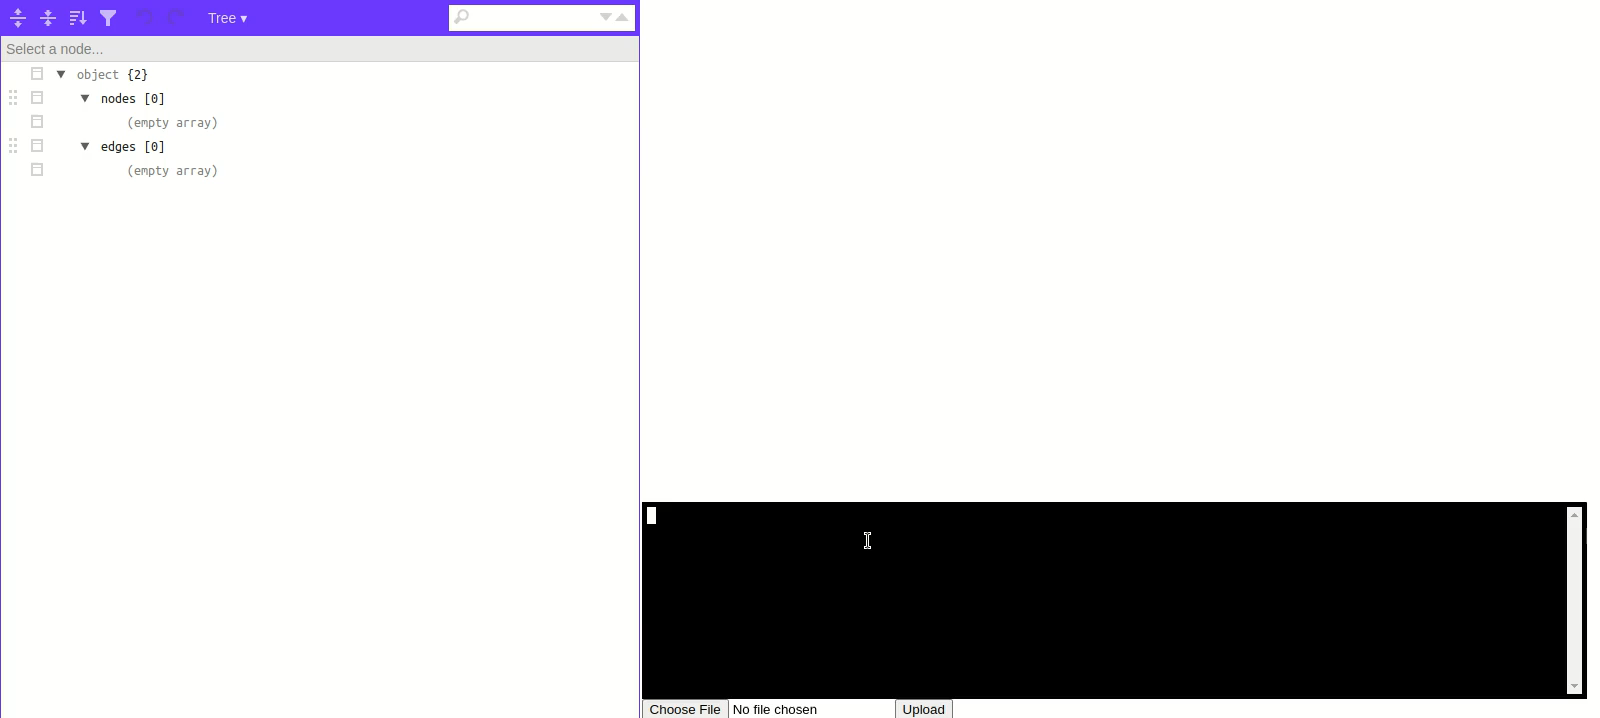
\includegraphics[width=\textwidth]{videos/thumbnail.png}}{videos/mcas_presentation.mp4}
        %     \end{center}
            
        % \end{frame}

 
	% \subsection{Attack/Defense scenarios integration}
	% \begin{frame}{Attack/Defense scenarios integration}
 %            {Integration approach}

 %            A high-level manual approach to integrate MITRE ATT\&CK information as an AD tree to formalize actions to be played in a scenario through the simulator.

 %            \begin{enumerate}
            
 %                \item Identify relevant tactics and techniques and procedures from MITRE ATT\&CK for an Advanced Persistent Threat (APT);
                
 %                \item Link tactics together and associated techniques, sub-techniques and procedures to create a scenario that describes how the APT group could attack the networked system;
            
 %                \item Establish an AD tree with tactics as top action goals while techniques, sub-techniques and procedures are in the lower part of the tree;
            
 %                \item Decorate the attack nodes with the MITRE ATT\&CK detection and mitigations.
                
 %            \end{enumerate}

        % \end{frame}


\AtBeginSection[]{
	\begin{frame}
		\frametitle{}
		\tableofcontents[currentsection]
	\end{frame}
}

%%%%%%%%%%%%%%%%%%%%%%%%%%%%%%%%%%%%
 
 \section{Case study}
	
	\subsection{Experimental setup}
	\begin{frame}{Experimental setup}
		{Network topology}

        Based on GALLIUM APT tactics we proposed a small company like networked environment:
        \begin{itemize}
            \item The cyber-attacker agents are initially deployed on At1 and At2 and the cyber-defender agents are deployed on WS and DB.
            \item The ultimate attackers' goals is to get data from the DB server and installing one spyware on the printer server PS.
        \end{itemize}

        \begin{figure}
            \centering
            \includesvg[width=0.65\linewidth]{figures/topology.svg}
            \caption{Proposed small-scale company network topology}
            \label{fig:scenario_network_topology}
        \end{figure}
 
	\end{frame}

    
	\begin{frame}{Experimental setup}
		{Attack/defense scenario}

        \vspace{-0.15cm}

        \begin{figure}
            \centering
            \includesvg[width=0.4\linewidth]{figures/ADTree.svg}

            \vspace{-0.2cm}
            
            \caption{An overview of the proposed attack/defense AD Tree}
            \label{fig:ADTree}
        \end{figure}
 
	\end{frame}


	\begin{frame}{Experimental setup}
		{Agent behavior implementation}

            \begin{block}{Random approach}
                \begin{itemize}
                    \item The agents only choose their actions by exploring the whole action space without any criteria until reaching the goal
                    \item Allows getting a benchmark of unexpected edge failure cases and to compare with other types of agent.
                \end{itemize}
            \end{block}

            \begin{block}{Decision Tree (DT) approach}
                Reference when cyber-attackers or cyber-defenders already know the best action to take as the role of each agent is defined by a DT.
            \end{block}

            \begin{block}{Multi-Agent Reinforcement Learning (MARL) approach}
                Q-Learning~\cite{CWatkins1992} with curriculum learning for first the attackers learn how to attack before adding defenders.
            \end{block}
 
	\end{frame}


 	\subsection{Results and discussion}

 	\begin{frame}{Results and discussion}
		{}

        \begin{itemize}
            \item After several iterations, chosen action paths by the attackers tend to be as efficient as the DT paths.
            \item When adding the defenders, we verified the attackers to be less and less able to reach the ultimate goal.
        \end{itemize}

        \begin{figure}
            \centering
            \includesvg[width=0.75\linewidth]{figures/graphs.svg}

            \vspace{-0.2cm}
            
            \caption{An evolution of the rewards average according to episodes in small-scale tests with MARL and Decision Tree Approaches with inactive cyber-defense
            }
            \label{fig:graphs}
        \end{figure}
 
	\end{frame}

\section{Conclusion et perspectives}
\begin{frame}{Conclusion et perspectives}
    {}

    \begin{prosblock}{\textbf{Contribution fondamentale} : AOMEA}
        \textbf{AOMEA} : assistance conception avec MARL et un modèle organisationnel.
    \end{prosblock}

    \begin{prosblock}{\textbf{Contribution pratique} : PRAHOM}

        \begin{itemize}
            \item \emph{Wrapper PRAHOM PettingZoo} comme preuve de concept pour l'application pratique d'AOMEA ;
            \item Permet d'obtenir certaines OS (Organizational Specifications) qui satisfont les contraintes de conception et permettent d'atteindre des objectifs donnés.
        \end{itemize}

    \end{prosblock}

    \begin{alertblock}{Perspectives}
        \emph{PRAHOM} utilise les historiques pour reconstruire des comportements collectifs $\rightarrow$ \textbf{difficile}
        \begin{itemize}
            \item Rendre inférence de Spec. Org. plus robuste ;
            \item \textit{Simulation-to-reality gap} $\rightarrow$ Auto-encoder + LSTM pour modélisation environnement
            \item Explorer les travaux récents en MARL, tels que \textbf{l'apprentissage hiérarchique} ;
            \item LLM pour des descriptions textuelles complémentaires des OS définies par les historiques.
        \end{itemize}
    \end{alertblock}

\end{frame}


\appendix
%\setbeamertemplate{headline}{}
\setbeamertemplate{mini frames}{}

% \AtBeginSection[]{
% 	\begin{frame}
% 		\frametitle{}
% 		\tableofcontents[currentsection]
% 	\end{frame}
% }

% %%%%%%%%%%%%%%%%%%%%%%%%%%%%%%%%%%%%

\section*{\phantom{Thanks}}

\begin{frame}{}

  \vspace{6ex}

  \centering
  {
    \Huge
    \emph{Thank You}
  }

  \vspace{6ex}

  \begin{columns}

    \hspace{-27ex}

    \begin{column}{0.5\textwidth}
      \raggedleft
      {\Large Demo video $\Longrightarrow$}
    \end{column}

    \hspace{-12ex}

    \begin{column}{0.5\textwidth}
      
\includegraphics[width=0.5\linewidth]{figures/demo_qr_code.png}
    \end{column}

  \end{columns}

  \vspace{3ex}

  \centering
  {\Large
    \url{https://t.ly/4JBxr}
  }

\end{frame}

% \AtBeginSection[]{
% 	\begin{frame}
% 		\frametitle{}
% 		\tableofcontents[currentsection]
% 	\end{frame}
% }

% %%%%%%%%%%%%%%%%%%%%%%%%%%%%%%%%%%%%

\section*{\phantom{References}}

\begin{frame}[allowframebreaks]{References}{}
    
    % \bibliographystyle{plain}
    % \bibliography{local_references}
        
    \printbibliography

\end{frame}

\end{document}

